%----------------------------------------------------------------------------------------
%	METODE
%----------------------------------------------------------------------------------------
\section*{METODE PENELITIAN}

Penelitian yang dilakukan mengikuti kaidah pengembangan sistem \textit{prototyping}. Model \textit{prototyping} terdiri dari beberapa tahapan yaitu komunikasi (pengumpulan kebutuhan), perencanaan dan pemodelan cepat, pembuatan \textit{prototype}, pengembangan sistem serta pengiriman hasil dan umpan balik (\textit{deployment delivery} dan \textit{feedback} atau evaluasi) (\cite{Pressman2010}). Gambar \ref{fig:tahapan} menunjukan tahapan proses pada metode \textit{prototype}.

\begin{figure}[h!] % Gunakan \begin{figure*} untuk memasukkan Gambar
\centering
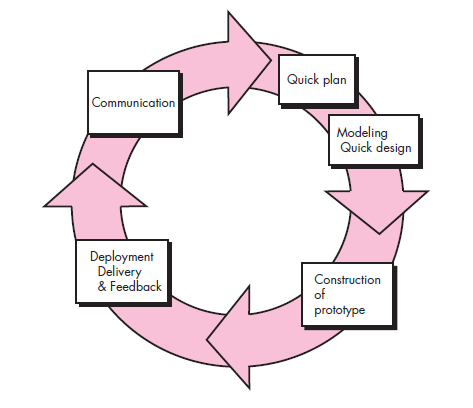
\includegraphics[width=200pt]{kolokium_contoh_gb1.png}
\caption{Tahapan proses penelitian (\cite{Pressman2010})}
\label{fig:tahapan}
\end{figure}

\subsection*{Pengumpulan Kebutuhan}

Tahapan ini mendefinisikan kebutuhan keseluruhan sistem. Mengidentifikasi proses bisnis dan garis besar sistem yang akan dibuat. Jenis pakan dan kebutuhan nutrisi pada hewan ternak didefinisikan pada tahapan ini. Data kandungan nutrisi pakan dan kebutuhan nutrisi hewan ternak yang digunakan sebagian acuan diperoleh dari NRC (1996).

\subsection*{Perancangan dan Pemodelan}

Menurut \citeauthor{Pressman2010} (\cite*{Pressman2010}) pada tahap ini dilakukan perancangan dan pemodelan sistem. Perancangan dan pemodelan yang dibuat disesuaikan dengan kebutuhan sistem yang telah didefinisikan pada tahap sebelumnya. Perancangan dibuat dalam bentuk gambaran antarmuka sistem serta input yang dibutuhkan dan output yang akan dihasilkan. Pembuatan model pada tahapan ini menggunakan pemrograman linier dengan metode simpleks. Pemrograman linier merupakan metode matematika dalam mengalokasikan sumber daya yang terbatas untuk mencapai suatu tujuan seperti memaksimumkan keuntungan atau meminimumkan biaya. Pemrograman linier banyak diterapkan dalam masalah ekonomi, industri, militer dan sosial. Dalam formulasi ransum dapat digunakan untuk mendapatkan harga seminimal mungkin (\cite{Wirdasari2009}). Penelitian \citeauthor{Hidayat2013} (\cite*{Hidayat2013}) menjelaskan persamaan matematis pemrograman linier bertujuan untuk memaksimumkan dapat dilihat pada persamaan dibawah ini.\\

Fungsi tujuan : \\
Z = c_{1}x_{1}+c_{2}x_{2}+...+C_{n}x_{n}\\

Dengan fungsi kendala:\\
a_{11}x_{11} + a_{21}x_{21} + ... + a_{n1}x_{n1} \leq  b1\\
a_{12}x_{12} + a_{22}x_{22} + ... + a_{n2}x_{n2} \leq  b2\\
..\\
..\\
a_{1m1}x_{1m} + a_{2m}x_{2m} + ... + a_{nm}x_{nm} \leq  bm\\
x_{1},x_{2}, ... , x_{n} \geq 0\\

Dimana, Z merupakan harga ransum yang diperoleh, c adalah harga bahan makanan yang digunakan, x adalah bahan makanan yang digunakan, a adalah kandungan nutrisi bahan makanan, b adalah standar kebutuhan nutrisi, dan m, n merupakan iterasi.\\
Menurut \citeauthor{Hidayat2013} (\cite*{Hidayat2013}) pemrograman linier memiliki syarat, yaitu:
\begin{enumerate}[noitemsep] 
	\item[a] Pemrograman linier harus memiliki fungsi tujuan (\textit{objective function}) berupa garis lurus dengan persamaan fungsi Z atau f(Z), c adalah \textit{cost coefficient}
	\item[b] Harus ada kendala (\textit{constraints}), yang dinyatakan garis lurus, dimana a = koefisien input-output dan b = jumlah sumber daya yang tersedia. 
	\item[c] Nilai X adalah positif atau sama dengan nol. Tidak boleh ada nilai X yang negatif.
\end{enumerate}
Pemrograman linier dapat digunakan untuk menentukan campuran makanan ternak yang efisien, praktis dan relatif mudah digunakan. Sesuai definisi, pemrograman linear adalah suatu teknik untuk menentukan kombinasi terbaik diantara pakan yang tersedia, yang mempunyai mempunyai kandungan nutrisi dan harga yang berbeda, dalam rangka untuk mendapatkan ransum dengan harga serendah mungkin. Hasil dari formulasi tersebut tergantung pada nilai yang digunakan untuk : 1) kandungan nutrisi dan spesifikasi lainnya yang diperlukan dalam ransum, 2) komposisi nutrisi dari bahan pakan yang dipilih, dan 3) unit harga dari tiap bahan pakan yang digunakan. Meminimumkan harga pakan akan menjadi fungsi tujuan dari model program linear, dengan kendala-kendala kandungan nutrisi dari setiap bahan pakan dengan sumber daya yang telah ditentukan (\cite{Hidayat2013}).

\subsection*{Pembuatan \textit{Prototype}}

Membangun \textit{prototyping} dengan mengimplementasikan hasil perancangan pada tahap sebelumnya. \textit{Prototyping} yang telah dibuat dilakukan evaluasi oleh pengguna dengan tujuan untuk mengevaluasi hasil pendefinisian kebutuhan yang telah dirancang pada tahap sebelumnya. Jika hasil evaluasi sudah sesuai dengan kebutuhan pengguna maka pengembangan dilanjutkan ke tahap selanjutnya, jika evalusai belum sesuai kebutuhan maka \textit{prototype} diperbaiki dengan mengulang langkah 1 dan 2. 

\subsection*{\textit{Deployment Delivery} dan \textit{Feedback}}

\textit{Prototype} yang sudah disepakati, dirancang dan dikembangkan ke dalam bahasa pemrograman yang sesuai. Sistem yang telah dibangun dilakukan evaluasi dan pengujian dengan menggunakan \textit{black-box testing}. Evaluasi bertujuan untuk mengetahui hasil dari optimasi pemrograman linier. Evaluasi dilakukan dengan melakukan perbandingan hasil dengan menggunakan aplikasi Winfeed. Evaluasi dilakukan dengan cara memberikan inputan pakan dan nutrisi yang sama antara sistem yang dikembangkan dengan aplikasi Winfeed. Hasil yang dibandingkan adalah presentase nutrisi berdasarkan kebutuhan jenis pakan dan perbedaan harga. Perbandingan tersebut akan menghasilkan selisih nilai. Hasil evaluasi yang baik adalah yang menghasilkan nilai selisih lebih kecil. Sistem yang telah diuji akan dikirimkan ke peternak dan siap digunakan.
